\documentclass[10pt, compress]{beamer}

\usetheme{m}

\usepackage{booktabs}
\usepackage[scale=2]{ccicons}
\usepackage{verbatimbox}

\title{Introduction to Dafny}
\subtitle{}
\date{\today}
\author{Lin Tzu-Chi}

\begin{document}

\maketitle

\begin{frame}[fragile]
  \frametitle{Dafny}

  Dafny is a imperative programming language with built-in annotations to prove correctness of code.
  
\end{frame}

\section{Basic Syntax}

\begin{frame}[fragile]
  \frametitle{Methods}
  
  \verb|method|s are functions in typical imperative languages.
  
  \begin{verbnobox}[\footnotesize]
  method Abs(x: int) returns (y: int)
  {
    if x < 0
      { return -x; }
    else
      { return x; }
  }
  \end{verbnobox}
  The input parameters are read only, and an implicit \verb|return| is added automatically at the end of a method, where the current values of return parameters are returned as-is.
\end{frame}

\begin{frame}[fragile]
  \frametitle{Methods}
  
  There can be multiple return values.
  \begin{verbnobox}[\footnotesize]
method MultipleReturns(x: int, y: int)
returns (more: int, less: int)
{
  more := x + y;
  less := x - y;
  // comments.
}
  \end{verbnobox}
\end{frame}

\begin{frame}[fragile]
  \frametitle{Pre- and Postconditions}
  \verb|ensures| annotates postconditions of a method for Dafny to check its correctness. 
  \begin{verbnobox}[\footnotesize]
method MultipleReturns(x: int, y: int)
returns (more: int, less: int)
  ensures less < x
  ensures x < more
{
    more := x + y;
    less := x - y;
}
  \end{verbnobox}	
  
Dafny rejects this program.
\end{frame}

\begin{frame}[fragile]
  \frametitle{Pre- and Postconditions}
  \verb|requires| annotates preconditions. It is the programmer's job to establish them.
  \begin{verbnobox}[\footnotesize]
method MultipleReturns(x: int, y: int)
returns (more: int, less: int)
   requires 0 < y
   ensures less < x < more
{
   more := x + y;
   less := x - y;
}

  \end{verbnobox}
  Dafny verifies this program successfully.

\end{frame}

\begin{frame}[fragile]
  \frametitle{Assertions}
  \verb|assert| is a keyword to place assertions in the moddle of a method.
  \begin{verbnobox}[\footnotesize]
// use definition of Abs() from before.
method Testing()
{
   var v := Abs(3);
   assert 0 <= v;
}
  \end{verbnobox}
\end{frame}

\begin{frame}[fragile]
  \frametitle{Assertions}

  The program:
  \begin{verbnobox}[\footnotesize]
var v := Abs(3);
assert v == 3;
  \end{verbnobox}
  would not be verified, because Dafny only knows the postconditions of \verb|Abs|, but nothing more.
\end{frame}

\begin{frame}[fragile]
  \frametitle{Assertions}
  To prove the assertion above, we can modify \verb|Abs| to provide more information.
  \begin{verbnobox}[\footnotesize]
method Abs(x: int) returns (y: int)
   ensures 0 <= y
   ensures 0 <= x ==> x == y
{
   // body as before
}
  \end{verbnobox}
\end{frame}

\begin{frame}[fragile]
  \frametitle{Functions}
  \begin{verbnobox}[\footnotesize]
function abs(x: int): int
{
   if x < 0 then -x else x
}
  \end{verbnobox}[\footnotesize]
  Unlike a method, which can have all sorts of statements in its body, a function body must consist of exactly one expression, with the correct type.
\end{frame}

\begin{frame}{Lists}
  \begin{columns}[onlytextwidth]
    \column{0.5\textwidth}
      Items
      \begin{itemize}
        \item Milk \item Eggs \item Potatos
      \end{itemize}

    \column{0.5\textwidth}
      Enumerations
      \begin{enumerate}
        \item First, \item Second and \item Last.
      \end{enumerate}
  \end{columns}
\end{frame}
\begin{frame}{Descriptions}
  \begin{description}
    \item[PowerPoint] Meeh.
    \item[Beamer] Yeeeha.
  \end{description}
\end{frame}
\begin{frame}{Animation}
  \begin{itemize}[<+- | alert@+>]
    \item \alert<4>{This is\only<4>{ really} important}
    \item Now this
    \item And now this
  \end{itemize}
\end{frame}
\begin{frame}{Figures}
  \begin{figure}
    \newcounter{density}
    \setcounter{density}{20}
    \begin{tikzpicture}
      \def\couleur{mLightBrown}
      \path[coordinate] (0,0)  coordinate(A)
                  ++( 90:5cm) coordinate(B)
                  ++(0:5cm) coordinate(C)
                  ++(-90:5cm) coordinate(D);
      \draw[fill=\couleur!\thedensity] (A) -- (B) -- (C) --(D) -- cycle;
      \foreach \x in {1,...,40}{%
          \pgfmathsetcounter{density}{\thedensity+20}
          \setcounter{density}{\thedensity}
          \path[coordinate] coordinate(X) at (A){};
          \path[coordinate] (A) -- (B) coordinate[pos=.10](A)
                              -- (C) coordinate[pos=.10](B)
                              -- (D) coordinate[pos=.10](C)
                              -- (X) coordinate[pos=.10](D);
          \draw[fill=\couleur!\thedensity] (A)--(B)--(C)-- (D) -- cycle;
      }
    \end{tikzpicture}
    \caption{Rotated square from
    \href{http://www.texample.net/tikz/examples/rotated-polygons/}{texample.net}.}
  \end{figure}
\end{frame}
\begin{frame}{Tables}
  \begin{table}
    \caption{Largest cities in the world (source: Wikipedia)}
    \begin{tabular}{lr}
      \toprule
      City & Population\\
      \midrule
      Mexico City & 20,116,842\\
      Shanghai & 19,210,000\\
      Peking & 15,796,450\\
      Istanbul & 14,160,467\\
      \bottomrule
    \end{tabular}
  \end{table}
\end{frame}
\begin{frame}{Blocks}

  \begin{block}{This is a block title}
    This is soothing.
  \end{block}

\end{frame}
\begin{frame}{Math}
  \begin{equation*}
    e = \lim_{n\to \infty} \left(1 + \frac{1}{n}\right)^n
  \end{equation*}
\end{frame}
\begin{frame}{Quotes}
  \begin{quote}
    Veni, Vidi, Vici
  \end{quote}
\end{frame}

\plain{Dark background}{\vspace{-2em}\begin{center}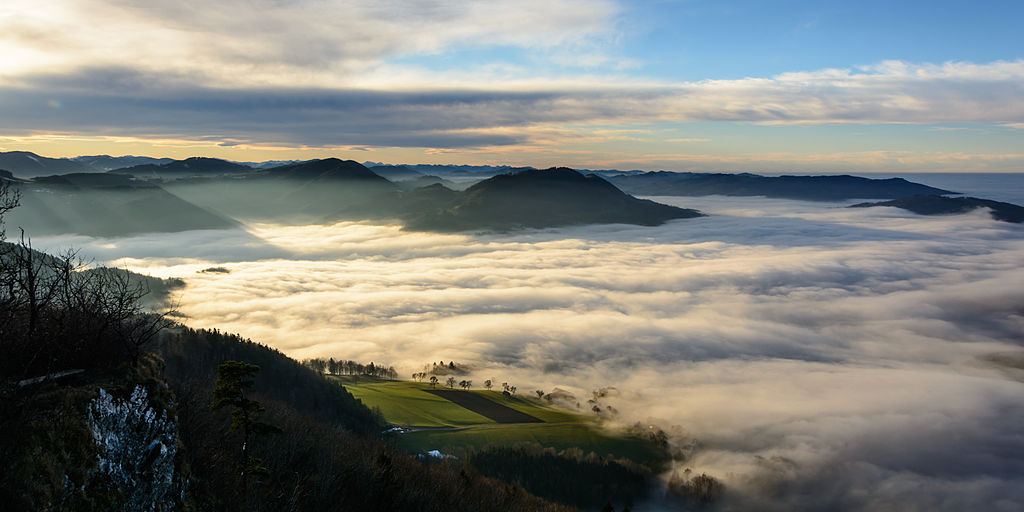
\includegraphics[width=\textwidth]{images/valley.jpg}\end{center}}

\section{Conclusion}

\begin{frame}{Summary}

  Get the source of this theme and the demo presentation from

  \begin{center}\url{github.com/matze/mtheme}\end{center}

  The theme \emph{itself} is licensed under a
  \href{http://creativecommons.org/licenses/by-sa/4.0/}{Creative Commons
  Attribution-ShareAlike 4.0 International License}.

  \begin{center}\ccbysa\end{center}

\end{frame}

\plain{}{Questions?}

\end{document}
